%%%%%%%%%%%%%%%%%%%%%%%%%%%%%%%%%%%%%%%%%%%%%%%%%%%%%%%%%%%%%%%%%%%%%%%%%%%%%%
\section{Comparisons to previous analyses}

Compared to previous analyses by the Boston University group \cite{MU2E_5391_PIPLUSENU}
and Purdue group \cite{MU2E_48165_PIPLUSENU}, this MC study finds significantly higher
background from the muon DIF.

We performed a detailed analysis of potential sources of the observed differences.
%
An immediate observation to make is that both groups tried to improve the efficiency
of the DIO simulation, and neither presented validation of the technique used.

%%%%%%%%%%%%%%%%%%%%%%%%%%%%%%%%%%%%%%%%%%%%%%%%%%%%%%%%%%%%%%%%%%%%%%%%%%%%%%
\subsection{Comparison to BU analysis (mu2e-5391) }

Table~\ref{table:comparison_to_bu} compares yield/POT of the \piplusenu\ and DIF events
reported by this analysis to the corresponding numbers reported in \cite{MU2E_5391_PIPLUSENU}.
The assumed signal window is 67.5-70 MeV/c.
W/o the degrader, the yields of the \piplusenu\ events are within 30\%,
however the integrals of the DIF contribution are different by an order of magnitude. In order to compare, a dataset with 3.5 mm Be degrader was simulated, as shown in figure~\ref{fig:bu_comparison}. The reduction in yield is similar.

\begin{figure}[H]
  \begin{tikzpicture}
    \node[anchor=south west,inner sep=0] at (0,0.) {
      % \node[shift={(0 cm,0.cm)},inner sep=0,rotate={90}] at (0,0) {}
      \makebox[\textwidth][c] {
        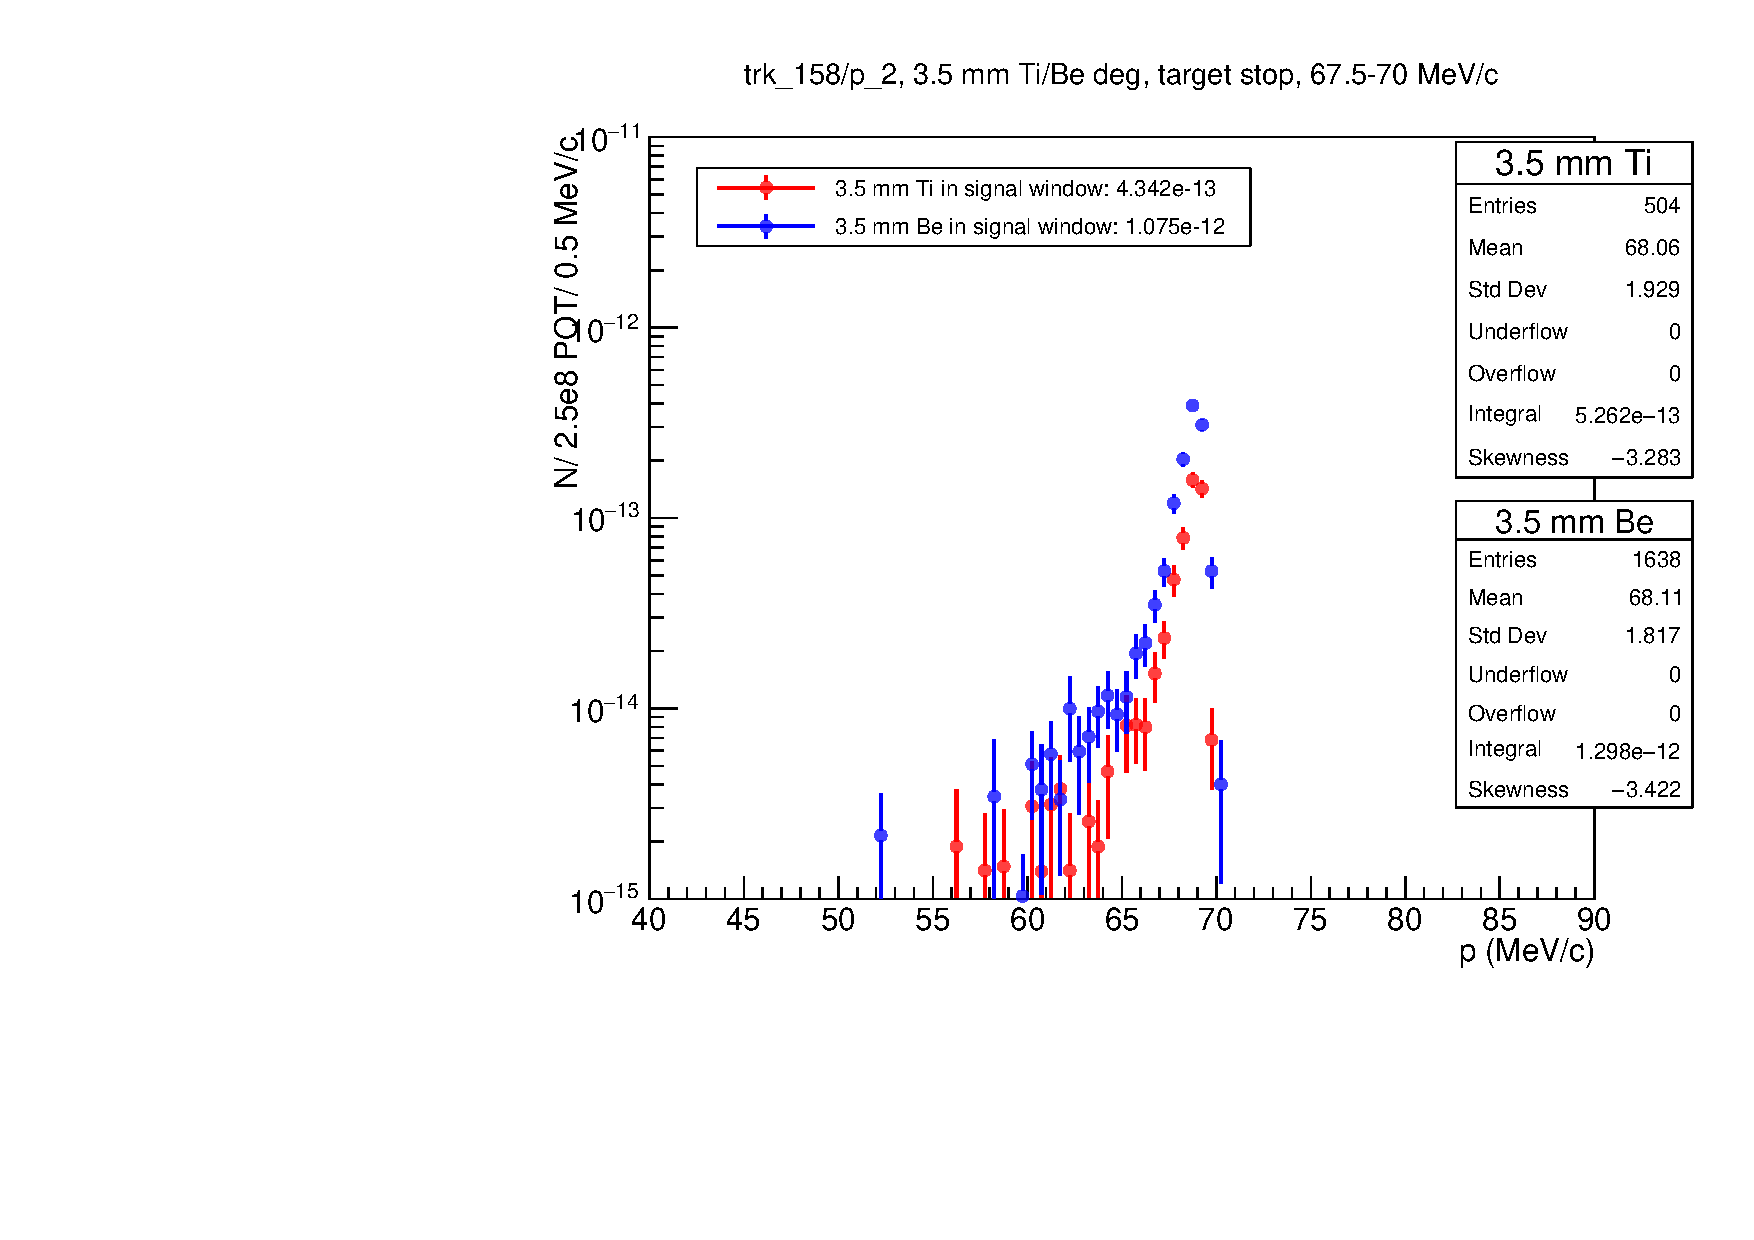
\includegraphics[width=0.7\textwidth]{pdf/figure_00405}
      }
    };
  \end{tikzpicture}
  \caption{
    \label{fig:bu_comparison}
  }
\end{figure}

{\red
  comparison for the 3.5 mm Be degrader - Sridhar
}
\begin{table}[H]
% \begin{tabularx}{1.0\textwidth} {|X|c|c|}  %
  \begin{tabularx}{0.7\textwidth} {|l|c|c|c|}  %
% \begin{tabular}{1.0\textwidth} {|l|l|}  %
    \hline
    channel     & degrader thickness &  mu2e-5391           &       this analysis       \\
    \hline                                                                     
    \piplusenu\ & none               &  $2.4 \times 10^{-12}$ &  $ 1.9 \times 10^{-12}$    \\
    \piplusenu\ & 3.5 mm             &  $1.9 \times 10^{-12}$ &  $ 1.1 \times 10^{-12}$    \\
    \hline                                                                     
    DIF         & none               & $1.2 \times 10^{-11}$ &  $1.7 \times 10^{-10}$      \\
    \hline
  \end{tabularx}
  \caption{
    \label{table:comparison_to_bu}
    Comparison of the yield/POT of the \piplusenu\ and DIF events reported by this analysis
    to the yields reported in mu2e-5391, The assumed signal window is 67.5-70 MeV/c.
  }
\end{table}


%%%%%%%%%%%%%%%%%%%%%%%%%%%%%%%%%%%%%%%%%%%%%%%%%%%%%%%%%%%%%%%%%%%%%%%%%%%%%%
\subsection{Comparison to the analysis by Purdue group (mu2e-48165)}

To improve the DIF simulation efficiency, the analysis by Purdue group \cite{MU2E_48165_PIPLUSENU}
used the technique introduced in \cite{MU2E_41916_KRZYSZTOF}.
However the authors also claimed to use the DIF event weights varying from one event to another
and defined by the individual muon decay probability, 
That looks inconsistent, as the technique used results in a constant event weight,

Comparisons of the \piplusenu\ and DIF event yields for the Ti degrader thicknesses of
3 mm and 4 mm within the momentum window of 68-70 MeV/c is presented
in Table~\ref{table:comparison_to_purdue}.

The yield of \piplusenu\ events reported in mu2e-48165 is systematically higher than in the
present study. Given low statistics, the reported DIF yields seem to be in the same ballpark.


\begin{table}[H]
% \begin{tabularx}{1.0\textwidth} {|X|c|c|}  %
  \begin{tabularx}{0.7\textwidth} {|l|c|c|c|}  %
% \begin{tabular}{1.0\textwidth} {|l|l|}  %
    \hline
    channel     & degrader thickness &  mu2e-48165         &       this analysis        \\
    \hline                                                                     
    \piplusenu\ & 3 mm   & $(9.2 \pm 0.11) \times 10^{-13}$ &  $ 4.8 \times 10^{-13}$     \\
    \piplusenu\ & 4 mm   & $(4.4 \pm 0.1) \times 10^{-13}$  &  $ 3.2 \times 10^{-13}$     \\
    \hline                                                                     
    DIF         & 3 mm   & $(4.8 \pm 1.4)\time 10^{-13}$    &  $3.8 \times 10^{-13}$      \\
    DIF         & 4 mm   & $(1.1 \pm 0.4)\time 10^{-13}$    &  $3.8 \times 10^{-13}$      \\
    \hline
  \end{tabularx}
  \caption{
    \label{table:comparison_to_purdue}
    Yield/POT comparison of the  \piplusenu\ and DIF events to the analysis of mu2e-48165,
    The comparison is performed for the signal momentum window of 68-70 MeV/c, defined in mu2e-48165.
  }
\end{table}
